\section{Space-based Actuation}
\label{sec:actuation_space}

% explicar brevemente patrones
% requirements: sistema de suscripciones (out of the scope)
% escenario de ejemplo en Ubicomp


In space-based computing, participants coordinate by reading and writing in a shared \Space{}.
This encourages an uncoupled communication between applications using the same \Space{}.


This section analyses how to achieve this uncoupled communication.
Section~\ref{sec:ts_patterns} briefly describes \acl{ts}'s most common application patterns. % according to the classification of \citet{freeman_javaspaces_1999}.
Section~\ref{sec:envisaged_scenarios} uses some of these patterns to show how to build two sample \ac{ubicomp} scenarios.
These scenarios help us to identify some additional requirements the middleware should fulfil.
Section~\ref{sec:notification} presents these requirements. % realmente sólo es uno: suscripción
Finally, Section~\ref{sec:actuation_scn1} explains how to implement the baseline scenario according to the space usage patterns. % más que usage pattern, igual es app pattern



\subsection{Application Patterns for \aclp{ts}}
\label{sec:ts_patterns}

According to \citet{freeman_javaspaces_1999}, there are four main application patterns which can be used in \ac{ts}:

\begin{description}
  \item[Replicated-worker pattern.] In this pattern, there is a master process and many worker processes able to compute the same task.
				    %% REDUCIENDO esto: %%
%				    The master takes a problem and divides it in tasks which are solved by any of the workers.
%				    More concretely the pattern is composed by the following steps:
% 				    \begin{enumerate}
% 				      \item The master divides a problem up into smaller tasks.
% 				      \item It writes them in the space.
% 				      \item Any of the many workers takes a task.
% 				      \item That worker computes the task.
% 				      \item It writes the result of that computation.
% 				      \item The master collects the results for the tasks it wrote.
% 				      \item Once the master has all the results, it combines them into a meaningful overall solution.
% 				    \end{enumerate}  
				    The master takes a problem, divides it into smaller tasks, and writes them tasks into the space.
				    Any available worker takes a task, processes it, and writes the result back into the space.
				    When all the workers have written their results, the master takes these results and combines them into a meaningful overall solution.
				    %Note that the workers accept new tasks whenever they are available and able to work.
				    %Therefore, while a worker is busy computing a big task, another one can solve many small tasks.
				    %In other words, this pattern naturally \emph{balances the load} on the space.
				    %Besides, it is \emph{scalable} since we can add more workers running in more machines without rewriting our code.
				    This pattern is scalable and naturally balances the load on the space.
  \item[Command pattern.] This pattern encapsulates the behaviour into the tuples shared in the space.
			  Therefore, it requires 
			  \begin{enumerate*}[label=\itshape(\arabic*\upshape)]
			    \item to share behaviour through the space, and
			    \item any generic worker to be able to compute the behaviour.
			  \end{enumerate*}
			  % nosotros pasamos de este jaleo
			  %For instance, a graph in \ac{tsc} could include code in an interpreted programming language. % elucubrar sobre esto sólo liaría
			  %In that way, a generic worker application can compute whatever code other processes define and share through the space.
			  %This pattern is only possible in \aclp{ts} where the behaviour can be described generically (e.g. in object-oriented \acp{ts}).
			  %Furthermore, the tasks to be performed over \ac{ubicomp} environments are not generically processable by any node.
			  %In contrast, each device is responsible of managing its own actuators on behalf of the rest.
			  %Therefore, this pattern will not be considered.
  \item[Marketplace pattern.] In this pattern, producers (or sellers) and consumers (or buyers) of resources interact to find the best deal. % TODO cita TripCom?
			  %It should be noted that the resources are products or services which can be bought and sold.
			  %Therefore, it is not applicable to the environments considered. % o use cases
			  %esto está relacionado con el paper aquel de TripCom y con el de Simon de hace un año en WoT
  \item[Specialist patterns.] In contrast to the replicated-worker pattern, in this pattern, each worker is specialized.
                              Therefore, each worker performs a particular task.
                              \citeauthor{freeman_javaspaces_1999} enumerate three subtypes:
			      \begin{description}
				  \item[Blackboard pattern.]
					It associates the concept of the space to a \emph{blackboard}.
					Following this analogy, the master is associated with a teacher, tasks with \emph{problems} and the specialized workers with \emph{students}.
					The blackboard pattern starts when the \emph{teacher} writes a \emph{problem} in the \emph{blackboard}.
					The \emph{students} observe the space and write their intention to contribute to solve the problem (i.e. \emph{raise their hands}).
					The \emph{teacher} selects to the expert which will make a modification.
					After the modification, the \emph{teacher} decides if it found the solution or another \emph{student} should contribute.
				  \item [Trellis pattern.]
					In this pattern, the master arranges the problem into low-level, mid-level, and high-level pieces.
					The workers of each level benefit from the refined data provided by the immediate level below.
				  \item [Collaborative patterns.]
					It encompasses all the patterns which allow nodes to collaborate to complete a greater task (i.e. by creating a workflow).
					%They are specific to the domain so they cannot be generalized, but it includes all the patterns where the nodes collaborate to complete a greater task
					%(e.g. by creating a workflow).
			      \end{description}
\end{description}


% Voy preparando el terreno para que se vea que los primeros son más de computación y el otro de negociación
To summarize, the \emph{replicated-worker pattern} is centred in optimizing the computation by parallelising tasks.
The \emph{command pattern} can be seen as an abstraction of the latter where the behaviour is shipped in the tuples.
The \emph{marketplace pattern} allows negotiation of two entities through the space.
% Coño! pero si el especialista te permite colaborar...
Finally, the \emph{specialist pattern} allows nodes with distinct capacities to cooperate towards a common goal.


% Posibilidad: Un esquema dividido en 4 en el que aparecen todos los patrones explicados.
%   No es fácil mostrar el 2do y el 3ero.
%   Una intentona de estos y otros patrones inventados en Lancaster:
%      https://docs.google.com/a/deusto.es/document/d/1QXGsQ4-wAByc_ByQ-Tts-TSphSQAzfO_c3mcgoZdloc/edit


\subsection{Envisaged Scenarios}
\label{sec:envisaged_scenarios}

This section devises two stereotypical scenarios for home automation.
Section~\ref{sec:envisaged_scn1} presents a scenario which regulates the temperature of a smart environment (e.g. a home or office) according to the user preferences.
Section~\ref{sec:envisaged_scn2} describes a smart environment which warns the user using different mechanisms to help him avoid a sedentary lifestyle.


Both scenarios emphasize how devices can coordinate in a decoupled mode using the patterns seen in the previous section. % más de uno?
Specifically, we believe that the \emph{specialist patterns} fit the best to the needs of \ac{ubicomp} environments:
\begin{itemize}
  \item The devices in \ac{ubicomp} often serve to very specific and local needs.
        For example, let us imagine a mobile phone showing a message or an embedded device turning on the lights of a room.
        %Although there may exist some redundancy in the tasks which different nodes can be accomplish, the task are not nodes are not as interchangeable as in... son tareas simples, no necesitan optimizar ni lanzar muchas
  \item These tasks are usually lightweight. % do not require a lot of computation resources.
	% TODO primera vez que se habla de "task", comentar que para TripCom eran servicios web y que crearon un sistema (WXSW?)
        They intent to achieve concrete and simple goals which usually imply more I/O operations than processing ones.
\end{itemize}
Therefore, \ac{ubicomp} generally faces a problem of collaboration between nodes with different capacities.
In this problem, computation or negotiation aspects are secondary. % se entenderá a qué me refiero con computation??


\subsubsection{Scenario 1: Temperature Regulation}
\label{sec:envisaged_scn1}

The first scenario presents a room populated with several kind of sensors such as Oracle's SunSPOTs \citeweb{sunspot},
% TODO TODO TODO referenciar a la parte donde se hayan referenciado bien los dispositivos! (e.g. see ~\ref{environment})
% Para el resto proveer al menos una URL!
Digi's XBee sensors with an IP gateway,
the sensors on a KNX domotic bus \citeweb{knx}, and a fan connected to a FoxG20 \citeweb{foxg20} embedded platform as an actuator (see Figure \ref{fig:devices_scenario}).
In addition, an Android application \citeweb{android} semantically stores the temperature preferences of the user.


\InsertFig{devices_scenario}{fig:devices_scenario}{
  The devices used in the devised scenarios.
}{
}{0.7}{}


An independent node (i.e. the master node) continuously reads from the space % using \emph{read primitive}
\begin{enumerate*}[label=\itshape(\arabic*\upshape)]
  \item the room's temperature, and
  \item the user's desired temperature.
\end{enumerate*}
Note that the master node does not care about who exactly provides the temperature information.
It just takes the first available graph from the space.
When the second one is below the first one, it generates a ``\emph{decrease temperature during a certain period}'' task which can be consumed by different independent worker nodes.
In this case, the FoxG20 periodically checks for orders it can fulfil extracting them from the space. % consumes them with a \textit{take primitive}.
% zasca, acabamos de poner en bandeja que nos rechine lo de comprobar periodicamente



\subsubsection{Scenario 2: Sedentary Lifestyle Checker}
\label{sec:envisaged_scn2}

The second scenario presents an application which helps the user to avoid a sedentary lifestyle by giving him different warnings.
We consider the recommendation that states that an adult should walk at least 10.000 steps in an ordinary day \citep{tudor2002taking}.
Taking into account the expected steps which should have been completed at each moment of the day, the application generates different priority level messages.

There are several nodes involved in this task.
Each node runs on a device. % which belongs to a user.
First, an Android phone periodically updates the number of steps covered by a user that day \citeweb{pedometer}.
%Besides, it writes her profile, more important to this problem: her age. % simplificado un poquillo
Second, there is an undefined number of devices which know how to warn the user about her unhealthy behaviour.
Third, there is a node in charge of generating the warnings.


\medskip


The application follows the \emph{blackboard pattern}.
The node which generates the warnings resembles a \emph{teacher}.
Each warning for a user resembles a \emph{problem} for the students.
Finally, the \emph{students} are allegorically represented by the devices which can warn the user.
% IG: no es nada intuitivo. Leyendo despues lo entiendo, pero... es raro
% AG: reescrito para hacer ver que hablo de una metafora/analogía/alegoría


When the \emph{teacher} writes a warning for a user, the devices able to warn the user write information about themselves into the space.
This information helps the teacher to select the most appropriate \emph{student} for each task.
In this example, the devices write their ownership and the intrusiveness level of their warning method.
The \emph{teacher} reads these characteristics, chooses a \emph{student} to solve the \emph{problem} and updates the \emph{problem} to indicate the selection.
%If no device writes their characteristics, the \emph{teacher} can wait longer.
Then, the selected device takes any warning for it and warns the user. % no tiene respuesta
If the chosen device does not take the message in a time span, the \emph{teacher} can update the \emph{problem} with a new selection.


With this application, if the priority level is low, the user receives the warning in a less intrusive way.
For example, room's light brightness can be increased for low priority notifications, a Chumby \citeweb{chumby} can show an icon for normal priority ones and the user's mobile phone show directly the message when it is a high priority warning. % IG: yo anyadiria una tablita para los dos scenarios mostrando los actuadores y los niveles. Aqui esto me salta un poco de repente.
The remarkable characteristic of this mechanism is that the devices present in the environment at each moment can vary and the application will still fulfil its goal.




\subsection{Notification mechanism}
\label{sec:notification}


In the scenarios described in the previous section, some writings in the space trigger other node's action.
For example, a device must show a message whenever a new warning is written in the space. % e.g. a task or a result
To be aware of these writings, the node can either poll the space or rely on a notification mechanism. % async or blocking
Obviously, the later leads to a more efficient use of the network. % is closer to optimal and more scalable approach.


As a consequence, a notification mechanism is highly advisable to fulfil \ac{ts}'s application patterns in a distributed environment.
Although the implementation of this notification mechanism is out of the scope of this thesis,
% Hablar de requisitos, describir nuevas primitivas de suscripciones o alternativas de implementación
it should comply with the following aspects:
\begin{itemize}
  %  Debe permitir polling (sync), por ello proponemos nuevas primitivas: read_async y take_async.
  \item Do not substitute the pull-based search. % porque todavía puede ser interesante en otros casos
        The middleware must provide additional \emph{read} and \emph{take} primitives.
  % Se evalúan sobre el espacio, no sobre el outer-space. 
  \item Since the notification mechanism intends to allow coordination patterns,
        it must consider the knowledge from the \coordspace{}. % TODO comprobar que lo llamé así en el anterior capítulo
        In other words, knowledge from the \outerspace{} will not trigger notifications. % TODO usar constante para esto
  % Evaluarse cada X, no siempre que se escriba algo o se vuelve loco.
  \item The evaluation of the subscriptions must not interfere with the writing process (e.g. introducing a delay).
        Therefore, it must run asynchronously.
  % Debe ser sencillo de implementar por cualquier nodo. Para ello proponemos un mínimo contrato: callback URL.
  \item Ease its adoption by any type of computing platform.
	This can be achieved by reducing the requirements on the \emph{clients}.
        For instance, a callback \ac{url} passed during the subscription can represent a minimal contract between the client and the server. % no viceversa
  % Deben caducar para no mantener suscripciones de dispositivos que ya no existen.
  \item Provide additional subscription removal mechanisms.
	\ac{ubicomp} scenarios are composed by unreliable devices which may frequently join and leave the space.
	In this situation, the correct use of unsubscription primitives cannot be guaranteed.
	This may worsen the performance of the system with useless subscriptions from absent devices.
	Therefore, the device managing the subscriptions should adopt more proactive mechanisms.
	For example, it may let the subscriptions expire after a lifetime or remove them when it discovers the unavailability of a callback \ac{url}. % algo así como garbage collection
	% A) The subscriptions must expire.
        % The expiration will allow to delete subscriptions from absent devices. % no longer present devices
        % This also implies that clients are responsible for periodically updating their subscriptions.
        % B) Additional mechanism
        % For instance, a \emph{garbage collection} agent can check the availability of callback \acp{url}.
        % For unavailable callback \acp{url}, the subscriptions can be removed.
\end{itemize}


The main drawback of any subscription mechanism is that it breaks the \acl{rests} property of the \ac{rest} style.
According to Section~\ref{sec:network_properties}, this implies that network performance will improve at the cost of scalability, simplicity and reliability.



\subsection{Baseline Scenario}
\label{sec:actuation_scn1}

This section describes how to implement the baseline scenario using \ac{tsc}.
The implementation presents the following nodes:
\begin{enumerate}[label=\itshape(\Alph*\upshape)] % o \itshape(\Alph*\upshape~node)
  \item A node which reacts to the tasks written into a shared semantic space.
	The node running this implementation is aware of the tasks written into the space and changes the light's value accordingly. % esto es, se suscribe a ellas
	Figure~\ref{fig:flow_space_prov} shows the initialization of this node and the process performed when a graph is detected.
	
  \item A node which writes tasks into a shared semantic space describing its desire to change the light's value.
	Figure~\ref{fig:flow_space_cons} shows the actions taken by this node.
	As it can be seen, the process is divided in two temporarily independent processes.
	The first writes the task and the second processes the result whenever it is written in the space.
	
  \newcounter{enumNodes}
  \setcounter{enumNodes}{\arabic{enumi}}
\end{enumerate}

% In advance, we will refer to these nodes as "A" and "B" using the following commands:
\newcommand{\nodeProvSpace}{\emph{Node A}}
\newcommand{\nodeConsSpace}{\emph{Node B}}


\begin{figure}
        \centering
	\subfigure[figtopcap][\nodeProvSpace] {
                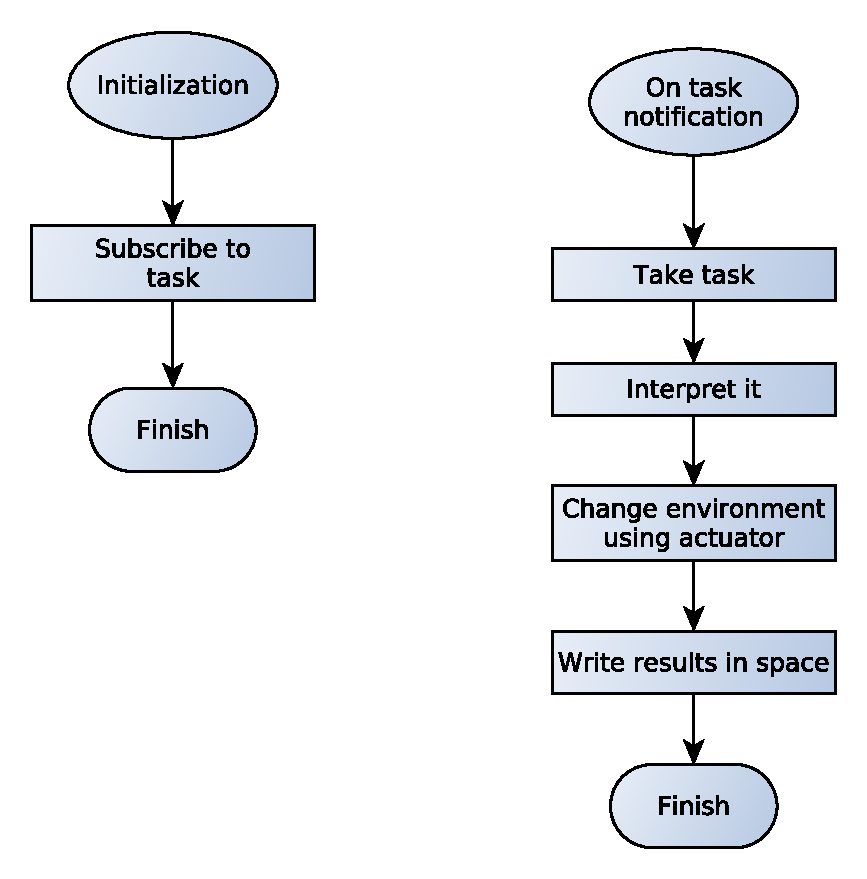
\includegraphics[width=0.45\linewidth]{flowSpaceProvider}
                \label{fig:flow_space_prov}
        }
	~ %add desired spacing between images, e. g. ~, \quad, \qquad etc.
          %(or a blank line to force the subfigure onto a new line)
	\subfigure[figtopcap][\nodeConsSpace] {
                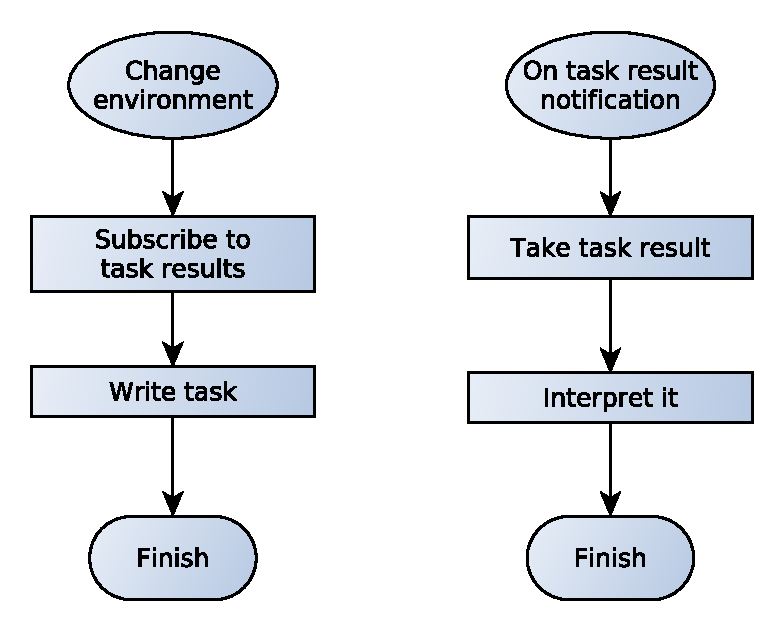
\includegraphics[width=0.45\linewidth]{flowSpaceConsumer}
                \label{fig:flow_space_cons}
        }
        \caption{Flow charts for \nodeProvSpace{} and \nodeConsSpace{}.}
        \label{fig:flow_space}
\end{figure}


\nodeProvSpace{} first subscribes to changes in the space (see Listing~\ref{lst:task_subscription}).
Then, \nodeConsSpace{} writes a task to be performed (see Listing~\ref{lst:task}) and subscribes to its result.
As a consequence of the writing, \nodeProvSpace{} reacts by taking the task, interpreting it, changing the environment through its actuator and writing the result.
Finally, \nodeConsSpace{} gets a notification of the written result, takes it and processes it.


\begin{listing}
  \expandafter\def\csname PY@tok@err\endcsname{}
{\small
\begin{Verbatim}[commandchars=\\\{\},numbers=left,firstnumber=1,stepnumber=1]
\PY{k}{select }\PY{n+nv}{?value }\PY{k}{where}\PY{p}{\PYZob{}}
\PY{n+nv}{  ?observation}\PY{o}{ a }\PY{n+na}{frap:Preference }\PY{p}{;}
	\PY{o}{a }\PY{n+na}{ssn:ObservationValue }\PY{p}{;}
	\PY{o}{dul:isClassifiedBy  }\PY{n+na}{ucum:lux }\PY{p}{;}
	\PY{o}{dul:hasDataValue }\PY{n+nv}{?value }\PY{p}{.}
\PY{p}{\PYZcb{}}
\end{Verbatim}
}

  \caption{Subscription to preferences written in the space.}
  \label{lst:task_subscription}
\end{listing}


% dar detalles de cómo se ha implementado
To simplify the implementation of the scenario, we consider a purely centralized space with a subscription mechanism.
% subscripciones SPARQL
This mechanism uses SPARQL \citeweb{sparql2008} and defines two different primitives.
The first one takes into account the knowledge from the last graph written to trigger the notifications.
% http://english.stackexchange.com/questions/2981/alternatives-to-computationally-expensive
The second primitive considers the knowledge from the whole space and hence is more computationally costly.

\begin{listing}
  \expandafter\def\csname PY@tok@err\endcsname{}
\begin{Verbatim}[commandchars=\\\{\},numbers=left,firstnumber=1,stepnumber=1]
\PY{n+nc}{:obsv} \PY{o}{a} \PY{n+na}{ssn:ObservationValue}\PY{p}{,} \PY{n+na}{frap:Preference} \PY{p}{;}
      \PY{n+nf}{dul:isClassifiedBy}  \PY{n+na}{ucum:lux} \PY{p}{;}
      \PY{n+nf}{dul:hasDataValue} \PY{l+m+mi}{21} \PY{p}{.}
\end{Verbatim}

  \caption{The preference is conceptually equivalent to a task.}
  \label{lst:task}
\end{listing}


% TODO Posiblemente haya que cargarse esto porque no encaja...

\subsubsection{Actuation Modelling}

% explain why like this? why not directly sensors/light?
The most abstract way to actuate on the environment would be to invoke a change referring to the sensed values.
For example, stating ``set \emph{Room A}'s light-level to 19 luxes''.
This would require the coordination of all the actuators which directly or indirectly affect this value.
Following the example, the lamps in \emph{Room A} and the curtains of \emph{Room A}'s windows should coordinate to give the exact desired value.


Even in this case, many other physical aspects would affect the value.
For instance, the daylight at each time of the day or the location of the light sensor.
As a consequence, we opt for clearly distinguishing between actuators and sensors.
In our implementations, the data measured by the sensors can only be indirectly affected by the actuators.


These indirect effects on the sensed values can be modelled for each actuator.
For example, to state that turning on a lamp increases the light measured by a sensor.
However, precisely anticipating the exact value of the new measure is difficult if not impossible due to the mentioned external physical conditions.
Considering this difficulty to predict their relationship and its tangential importance for the implementations, we simply ignore these relationships.
We assume that the consumer previously determined which actuators it should change to fulfil its initial abstract goal.


\subsubsection{Ontologies Used}

% Ontologies used
% explicar por qué hemos modelado así los escenarios?
The \emph{glue} between the two actuation worlds presented in this chapter is their data. % o between both approaches, o yo qué sé
Therefore, it must be modelled according to the same ontologies.
This section provides the rationale behind the selection of the ontologies we used.
Note that these ontologies are not the unique selection which could be made.
Neither does it pretend to be the best one.


% por qué con medidas?
To represent the value of a lamp actuator, we use the SSN ontology \citeweb{ssn}.
For example, we express that ``the lamp actuator has a light value of \emph{N} luxes''.
The SSN ontology is intended to describe measures for sensors, so its use for actuators can sound contradictory.
Note how the previous statement differs from ``the light sensed by a sensor located near the lamp has a value of \emph{N} luxes''.
However, to the best of our knowledge, there is no more widely-accepted ontology to specifically describe actuators.


% por qué uso preferencias?
The preferences ontology is another of the core ontology used in our implementations.
It is used to clearly distinguish between the value of an actuator and a consumer's intention or desire to change it.
A preference can turn into an actuator's new state, but it is not always necessarily true.
The actuator can discard a preference due to an usage policy, a malfunction or any other reason.

% por qué no se tienen en cuenta otras características como la localización o lo que sea => por simplificar
%   en el goal se podrían describir